% !TEX root = ../gnss_interference_resistant_thesis.tex
\documentclass[main.tex]{subfiles}

\begin{document}

\subsubsection{Spindulio formavimo matavimo stendas}\label{sec:beamform_meas_stand}

Spindulio formos matavimui naudojamas stendas pavaizduotas \ref{fig:beamform_stand}
pav. Pagrindiniai stendo elementai:

\begin{enumerate}
    \item HackRF siųstuvas, kuris generuoja CW signalą;
    \item 1x2 spinduolių sistema sudaryta iš GNSS signalams priimti skirtų antenų;
    \item Du HackRF koherentiniai imtuvai, susinchronizuoti anksčiau aptartais metodais;
    \item Siųstuvo stovas, kuris leidžia keisti siųstuvo kampą, spinduolių sistemos atžvilgiu;
\end{enumerate}

\begin{figure}[h]
    \begin{centering}
    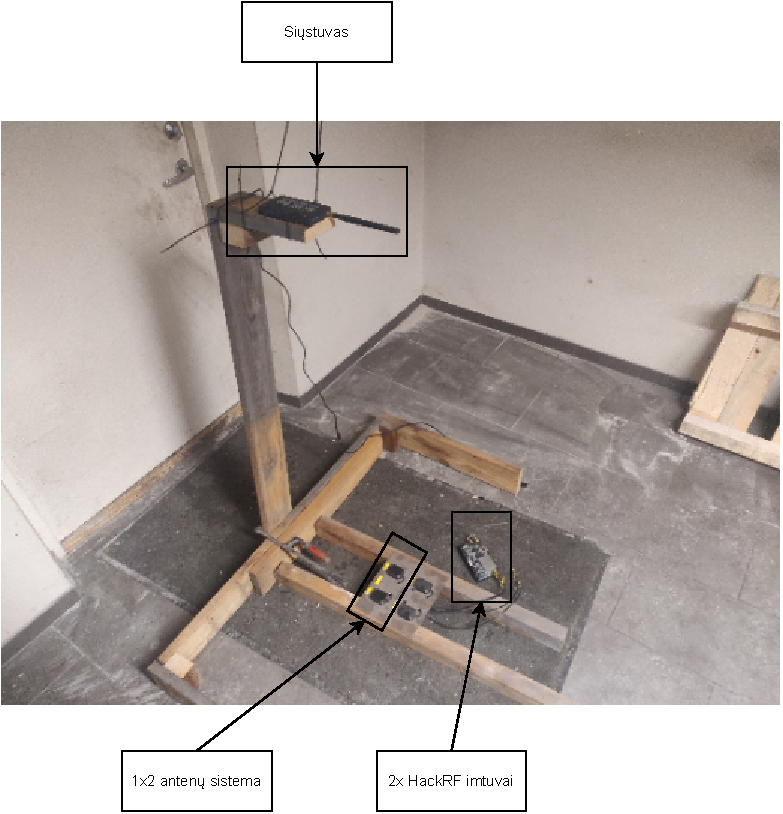
\includegraphics[scale=1.0]{drawings/beamform_stand.drawio}
    \par\end{centering}
    \protect\caption{\label{fig:beamform_stand}Spindulio formos matavimo stendas.}
\end{figure}

Matavimai stendu pradedami vertikalioje padėtyje, įjungiamas siųstuvas ir abu imtuvai.
Atliekant signalų koreliaciją priimtų iš atskirų antenų, patikrinama laikinė sinchronizacija
ir randamas fazių skirtumas, kuris yra išsaugomas ir pritaikomas vienam iš imtuvų.

Spinduolių diagrama matuojama skaičiuojant priimamo signalo stiprumą: atliekama FFT
transformacija ir matuojamas maksimumo dydis. Nuskaičius vieną tašką, siųstuvo stovas
yra pasukamas iki kito kampo. Kampas yra matuojamas pasinaudoju išmaniojo telefono
akselerometro pagalba. Išmatavus vieno spinduolio diagramą įjungiamas spindulio formavimas
(signalų sudėtis) ir vėl kartojamas matavimas keičiant vieno iš imtuvo fazę.

\end{document}